% !TEX root = ms.tex
\chapter{Plataforma de Desarrollo}

En este capítulo se desarrollarán algunas de las herramientas y recursos
utilizados mas relevantes a lo largo del proyecto

\section{Arch Linux}
El sistema operativo elegido para la placa en la que se desplegará la MCE es 
Arch Linux. La elección se fundamenta en su bajo coste computacional (lightweight), su
amplia compatibilidad con herramientas modernas de desarrollo, y su flexibilidad
para configuraciones personalizadas, lo cual resulta especialmente valioso
durante las fases experimentales del proyecto. Al tratarse de una distribución
minimalista, permite un mayor control sobre los paquetes instalados y el entorno
de ejecución, optimizando así los recursos del sistema.

Aunque el proceso de instalación y configuración de Arch Linux requiere
conocimientos intermedios en sistemas operativos, su adopción ofrece ventajas
significativas en términos de rendimiento, estabilidad y transparencia del
entorno. Además, la estructura del sistema facilita la automatización y el
despliegue de servicios relacionados con la MCE.

Cabe destacar que Arch Linux funcionará como sistema anfitrión (host) para la
ECM, desempeñando el rol de servidor para las Capas de Ejecución/Cognición. No obstante, 
el espacio de acciones (esto es, la máquina controlada) es compatible con otros 
sistemas operativos, como Windows, Ubuntu o Raspbian, lo que garantiza la 
interoperabilidad y flexibilidad del sistema en entornos heterogéneos.


\section{Kit de Desarrollo}
Para la implementación y validación de la MCE se ha optado por el uso del kit de
desarrollo IMX8MPEVK, el cual proporciona acceso completo al SoC i.MX 8M Plus,
que incorpora un microprocesador ARM Cortex-A53. Este kit permite realizar
pruebas exhaustivas sobre un entorno embebido realista, facilitando el
desarrollo, despliegue y evaluación del sistema en condiciones similares a las
de un producto final.

Aunque el coste del kit de desarrollo es elevado, el microprocesador utilizado
se encuentra disponible en el mercado por un rango estimado de 30 a 40 euros, lo
cual se ajusta a la filosofía de bajo coste del proyecto. El propósito del uso
de este kit es demostrar que la MCE puede ser ejecutada en un sistema basado en
un microprocesador accesible económicamente, validando así su viabilidad como
prototipo para futuras aplicaciones a escala, donde la arquitectura puede ser 
directamente integrada en el SoC i.MX sin necesitar del kit de desarrollo.

Se ha decidido utilizar un microprocesador en lugar de un microcontrolador por
dos razones fundamentales. En primer lugar, el proyecto requiere de un sistema
operativo completo que permita instalar y ejecutar múltiples herramientas de
desarrollo y control, muchas de las cuales no son compatibles con
microcontroladores tradicionales. En segundo lugar, el sistema debe ser capaz de
soportar operaciones complejas y arquitecturas cognitivas avanzadas, que exigen
una capacidad de procesamiento superior y una mayor flexibilidad en la gestión
de recursos.

\begin{figure}[!h]
    \centering
    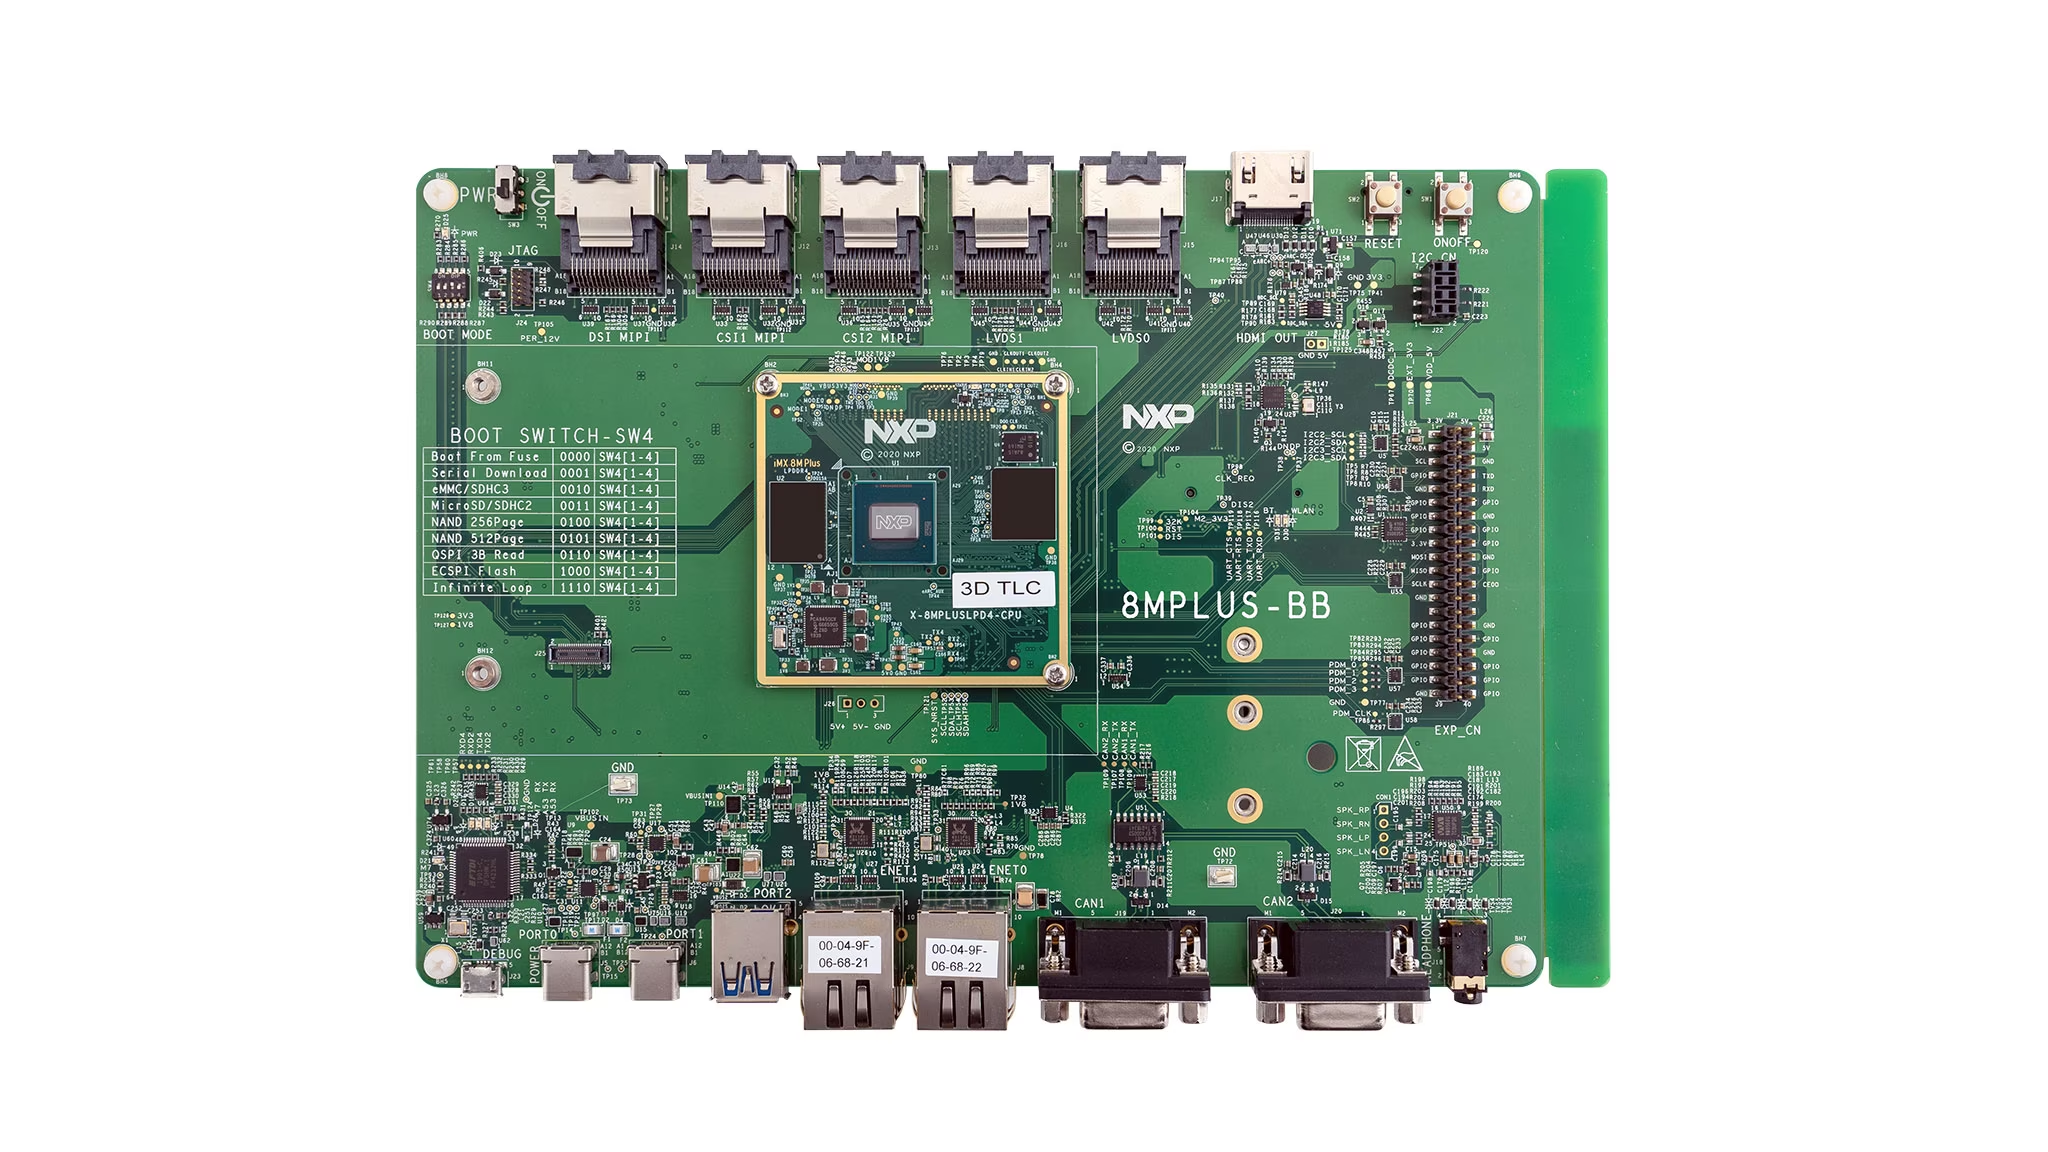
\includegraphics[scale=0.15]{figs/imx8mpevk.png}
    \caption{\small Kit de desarrollo IMX8MPEVK. Fuente: https://www.nxp.com/}
    \label{fig:imx8mpevk}
\end{figure}

\section{Python}
El lenguaje de programación elegido para el desarrollo de la MCE es Python, 
considerado actualmente el lenguaje de facto en el ámbito de la inteligencia
artificial. Esta elección responde tanto a su popularidad como a su ecosistema
maduro, que incluye una amplia gama de bibliotecas especializadas como
LangChain, MCP y FastAPI, fundamentales para la implementación modular y
conectada de arquitecturas cognitivas.

Adicionalmente, Python otorga la capacidad de diseñar sistemas complejos
de forma legible y mantenible. Características como la introspección dinámica,
el tipado flexible, y la posibilidad de realizar meta-programación permiten
definir estructuras adaptativas, propiedad que resulta esencial para un sistema 
como la MCE, donde los módulos no solo deben poder reemplazarse o ampliarse 
sin reestructurar el sistema completo sino que ademas deben poder configurarse 
de forma automática en tiempo real.

\section{Langchain/LangSmith}

Las bibliotecas LangChain y LangSmith constituyen elementos fundamentales para la
implementación y monitoreo de la MCE.

LangChain actúa como capa de abstracción que permite interactuar, de forma
unificada, con distintos modelos de lenguaje disponibles a través de API,
tales como los ofrecidos por Anthropic, OpenAI, Ollama, entre otros. Más allá
del acceso a modelos, LangChain proporciona un conjunto robusto de patrones de
diseño orientados a agentes, incluyendo sistemas de mensajería, mecanismos 
de prompting estructurado, modelos de memoria contextual y soporte para
grafos agénticos. Estas funcionalidades son esenciales para la construcción de
arquitecturas cognitivas de alto nivel, facilitando la organización jerárquica y
modular de los procesos cognitivos simulados por la MCE.

Complementariamente, LangSmith se integra como plataforma de observabilidad y
trazabilidad del sistema. Esta herramienta permite registrar, de manera no
intrusiva, el flujo completo de interacciones dentro de los agentes construidos
con LangChain. A través de su interfaz gráfica, es posible visualizar de forma
clara el comportamiento del sistema, incluyendo información crítica como la
latencia, el coste computacional, el número de llamadas a modelos y el flujo de
decisiones. Esta capacidad resulta especialmente útil durante las fases de
experimentación e iteración, ya que permite identificar cuellos de botella,
evaluar el rendimiento y realizar ajustes con mayor precisión.

\begin{figure}[!h]
    \centering
    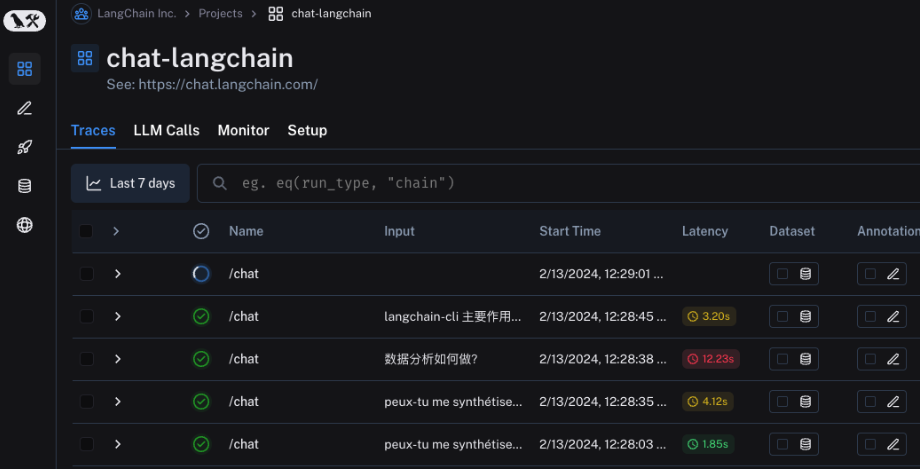
\includegraphics[scale=0.5]{figs/langsmith.png}
    \caption{\small Interfaz de depuración de LangSmith para componentes de LangChain. Fuente: https://docs.smith.langchain.com/}
    \label{fig:langsmith}
\end{figure}

\section{PyAutoGUI/Pynput}
Para habilitar la interacción directa entre la MCE y el sistema operativo del
cliente controlado, se emplean las bibliotecas PyAutoGUI y Pynput. 

Estas bibliotecas permiten tanto la captura de información contextual como la
manipulación activa del sistema, actuando como una interfaz sensorimotora entre
la arquitectura cognitiva y el entorno operativo. En concreto, PyAutoGUI se
utiliza principalmente en sistemas Windows y Pynput en entornos Linux, lo que
asegura una cobertura multiplataforma para la ejecución del sistema.

En el plano perceptivo, estas herramientas posibilitan la captura de capturas de
pantalla y el monitoreo de eventos del usuario, como movimientos
del ratón o pulsaciones de teclas. Estos datos perceptuales son enviados a las
capas cognitivas para su análisis e interpretación, actuando como entrada
sensorial del sistema.

De forma inversa, la capa de ejecución de la MCE puede controlar activamente el
entorno mediante simulación de entrada de teclado, clics de ratón o
desplazamiento del cursor, lo que permite ejecutar comandos, interactuar con
aplicaciones y realizar tareas definidas por el usuario. Este mecanismo
convierte a la MCE en un agente capaz de operar sobre sistemas externos de
manera autónoma y efectiva, sin requerir modificaciones en el sistema operativo
huésped.

\section{OpenCV / Pillow}

Dado que la MCE debe ser capaz de percibir e interpretar información gráfica del
entorno se integran las bibliotecas OpenCV y Pillow como herramientas fundamentales 
para el procesamiento de datos visuales.

Ambas bibliotecas permiten transformar la información gráfica capturada
en representaciones estructuradas que pueden ser utilizadas por la
capa cognitiva del sistema. En este contexto, se han empleado para tareas como
la detección y localización de iconos, la generación de regiones de interés
mediante bounding boxes, y el ajuste de calidad o resolución de las imágenes,
adaptando la información visual a formatos que resulten viables para su análisis
automatizado.

Adicionalmente, estas herramientas también han sido utilizadas como soporte 
para técnicas de OCR (reconocimiento óptico de caracteres), permitiendo 
extraer texto de elementos gráficos que luego puede ser interpretado y 
utilizado por los módulos cognitivos.


\begin{figure}[!h]
    \centering
    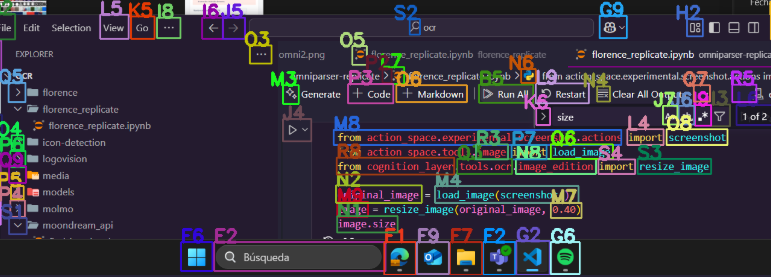
\includegraphics[scale=0.4]{figs/icon-detection.png}
    \caption{\small Detección de iconos detectados en pantalla usando OpenCV y Pillow. Fuente: Elaboración Propia}
    \label{fig:icon_detection}
\end{figure}

